\section{Introduction}

  \subsection{Qu'est ce qu'un utilisateur ?}
	
	C'est un compte permettant g�n�ralement une connexion (graphique ou console).
	
	Il est associ� sous UNIX � un num�ro qui est utilis� pour identifier les fichier et les r�pertoires
	
	Il est g�n�ralement associ� � la pr�sence d'un r�pertoire utilisateur qui lui appartient.



	Il existe des utilisateurs sp�ciaux qui n'ont pas de r�pertoire et/ou la connexion n'est pas possible.
	
	C'est le cas pour de nombreux serveurs qui fonctionnent ainsi pour des raisons de s�curit�.
	

\section{Gestion des utilisateurs}

  \subsection{Cr�er/supprimer un utilisateur}

	Pour cr�er un utilisateur, il suffit d'utiliser la commande \emph{adduser <utilisateur>} pr�c�d� de \emph{sudo}.
	
	Et apr�s il faut r�pondre aux questions, relativement simple.
	
	En effet la gestion des utilisateurs est r�serv� au super utilisateur.

	Pour supprimer un utilisateur, il faut utiliser \emph{deluser <utilisateur>} et de r�pondre aux questions.
		

  \subsection{Les fichiers de r�f�rence}
	
	Le fichier des utilisateurs est le fichier /etc/passwd.
	
	Le fichier des groupes est le fichier /etc/group.
	
	Le fichier des groupes est plus int�ressant car il permet de voir quels groupes contiennent quels utilisateurs.
	C'est utile par exemple pour copier les droits de l'utilisateur cr�� par d�faut par votre distribution.

	\textcolor{red}{Mais il faut �viter de manipuler directement ces fichiers car s'ils sont corrompus le syst�me d'authentification peut planter}

  \subsection{Gestion des groupes}
	
	Pour ajouter un groupe � un utilisateur, il faut utiliser la commande~:
	\emph{usermod -a -G <groupe> <utilisateur>}.
	
	Pour ajouter un groupe � un utilisateur, il faut utiliser la commande~:
	\emph{gpasswd -d <utilisateur> <group>}.
		

  \subsection{Nota bene}
	
	Les droits sont des num�ros.
	
	Si l'utilisateur pascal est 1001 sur un ordinateur et 1002 sur un autre ordinateur, alors
	si vous �changez les disques les fichiers ne seront pas reconnus comme pascal sur l'un
	ou l'autre des ordinateurs.
		

  \subsection{En mode graphique}
	
	Sous KDE, l'utilitaire KUser permet de le faire graphiquement comme system-config-users sous GNOME.
		

  \subsection{Sous GNOME 3}

\begin{center}
\begin{figure}
 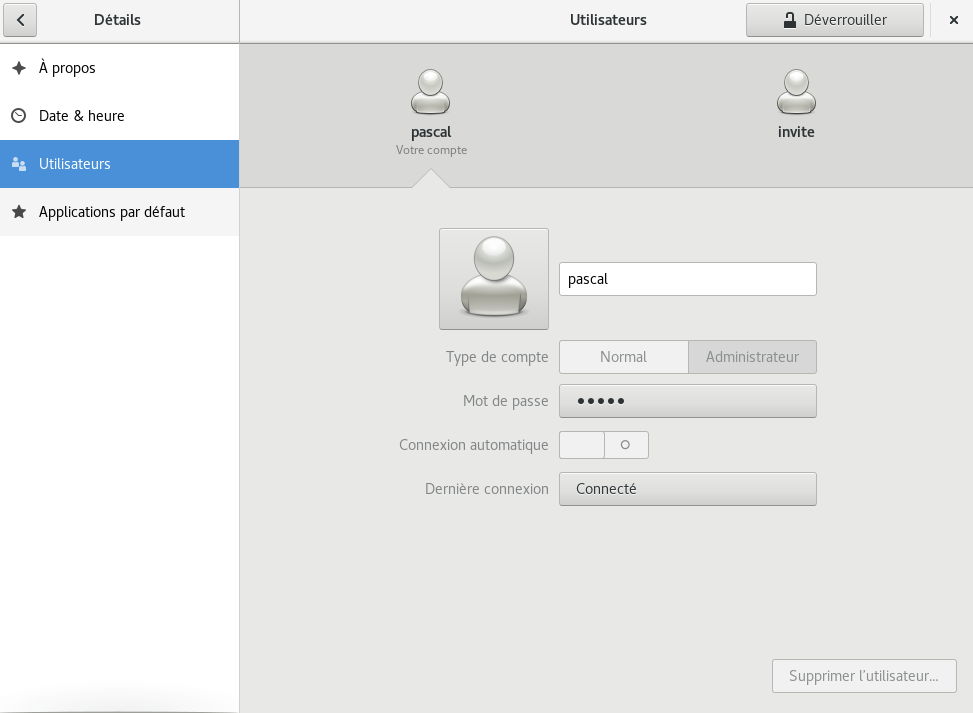
\includegraphics[scale=0.2]{Figures/Selection005}
	\caption{Utilisateurs dans le menu D�tails de l'application Param�tres}
\end{figure}
\end{center}
  


\begin{center}
\begin{figure}
 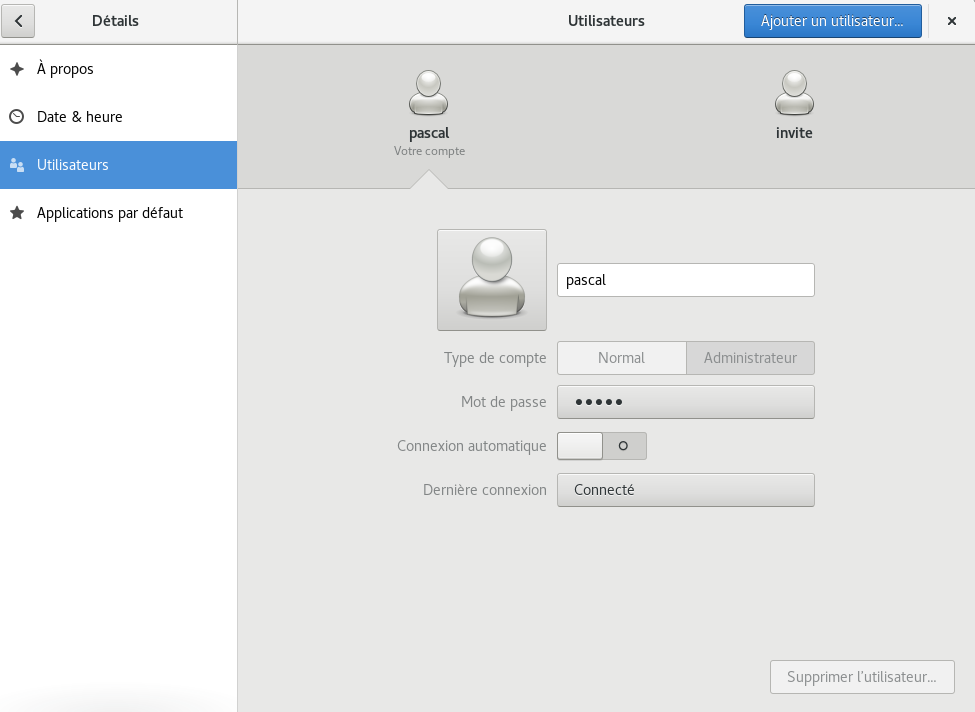
\includegraphics[scale=0.2]{Figures/Selection006}
	\caption{Utilisateurs, d�blocage avec le mot de passe}
\end{figure}
\end{center}
  



\begin{center}
\begin{figure}
 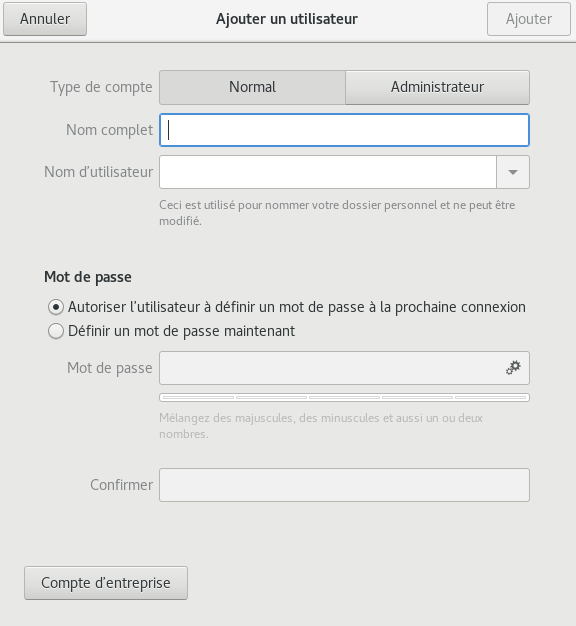
\includegraphics[scale=0.2]{Figures/Selection007}
	\caption{Utilisateurs, nouvel utilisateur}
\end{figure}
\end{center}
  

	
